\section{Geometric Representation}
Consider the unit square and its diagonal. The length of this diagonal is precisely $\sqrt{2}$, giving us our first geometric insight into the number's nature. Each digit in the binary expansion can be thought of as a geometric construction:

\begin{figure}[H]
\centering
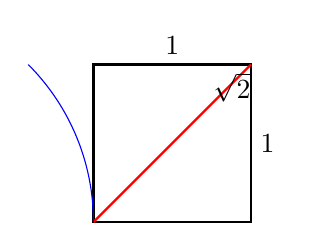
\begin{tikzpicture}[scale=2]
    % Unit square
    \draw[thick] (0,0) rectangle (1,1);
    % Diagonal
    \draw[red,thick] (0,0) -- (1,1);
    % Arc showing sqrt(2)
    \draw[blue] (0,0) arc (0:45:1.414);
    % Labels
    \node[right] at (1,0.5) {1};
    \node[above] at (0.5,1) {1};
    \node[above right] at (0.7,0.7) {$\sqrt{2}$};
\end{tikzpicture}
\caption{The fundamental geometric relationship of $\sqrt{2}$}
\end{figure}

\section{Binary Expansion and Geometric Approximation}
Each binary digit represents a halving of the previous geometric step. A run of zeros in the binary expansion signifies a period where our approximation maintains its position relative to $\sqrt{2}$ without requiring adjustment. Geometrically, this translates to:

$$\sqrt{2} = 1.011010100000100111100\ldots_2$$

\section{The Geometric Constraint}
The key insight comes from understanding why runs of zeros must be limited. Consider a rational approximation $\frac{p}{2^n}$ of $\sqrt{2}$. Geometrically, this represents a point on our binary grid. For any such approximation:

$$\left|\sqrt{2} - \frac{p}{2^n}\right| \geq \frac{1}{2^{2n}}$$

This inequality has a beautiful geometric interpretation: it represents the minimum "gap" that must exist between any rational approximation and $\sqrt{2}$.

\section{Connection to Zero Runs}
A run of $k$ zeros in the binary expansion at position $n$ implies an approximation accurate to $2^{-k}$ at that position. The geometric constraint above tells us this accuracy cannot exceed certain bounds, directly leading to the $\log_2(n)$ limit on zero runs.

\begin{figure}[H]
\centering
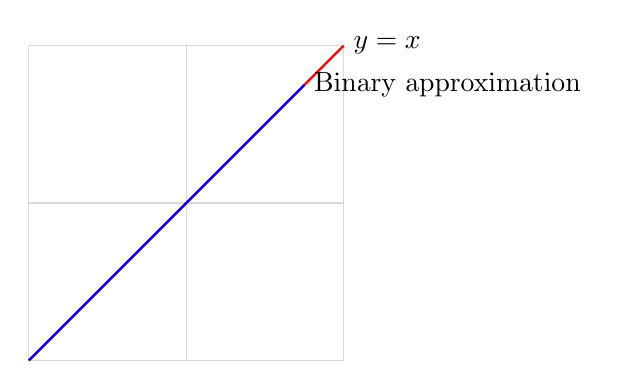
\begin{tikzpicture}[scale=2]
    % Grid
    \draw[gray!30] (0,0) grid (2,2);
    % Main diagonal
    \draw[red,thick] (0,0) -- (2,2);
    % Binary approximation steps
    \draw[blue,thick] (0,0) -- (1,1) -- (1.5,1.5) -- (1.75,1.75);
    % Labels
    \node[right] at (2,2) {$y=x$};
    \node[right] at (1.75,1.75) {Binary approximation};
\end{tikzpicture}
\caption{Binary approximation steps approaching $\sqrt{2}$}
\end{figure}

\section{Conclusion}
The geometric perspective provides intuitive understanding of why the binary expansion of $\sqrt{2}$ cannot have arbitrarily long runs of zeros. The fundamental relationship between the square and its diagonal, combined with the discrete nature of binary fractions, enforces this limitation.

